\chapter{Methodology}

\lettrine[
	nindent=0em, findent=0.5em, loversize=-0.12, lines=5
]{\initfamily{N}}{\bfseries\color{Blue}eural networks}\index{Neural network} are
notorious for being ``data hungry'', requiring a relatively large amount of
training data\index{Training data}, in order to unleash their full potential. As
such, to get a representative picture of the capabilities of the proposed
\gls{dl} framework, two large datasets\index{Dataset} are employed to train the
3D \gls{cnn}. The first one, is a subset of the \gls{uo} database\index{UO
database} \parencite{Boyd_2019}, and is used to verify the applicability of the
proposed pipeline, examining \ch{CO2} uptake. The second one, is the \glspl{cof}
database generated by \parencite{Mercado_2018}, and is employed to demonstrate the
transferability of the approach, examining \ch{CH4} uptake. Please note, that
these datasets are already labeled, and as such no molecular
simulations\index{Molecular simulations} were performed in this study to
generate the labels\index{Label} (gas uptakes)\index{Gas uptake} of the
materials. Information regarding the \gls{gcmc} calculations that were performed
to produced the labels, can be found in the original works.

\section{Datasets\index{Dataset}}
\label{sec:datasets}

\subsection{\Acrshortpl{mof} dataset}

The \gls{uo} database is composed of \num{324426} hypothetical
\glspl{mof}\index{Hypothetical MOFs}. Randomly selected subsets of size
\num{32432}, \num{5000} and \num{27438}, served as the training\index{Training
set}, validation\index{Validation set}\footnote{The validation set was used to
select the number of epochs, see Section \ref{subsec:preprocessing}.} and test
sets\index{Test set}, respectively. The absolute \ch{CO2} uptake at
\SI{298}{\kelvin} and \SI{0.15}{\bar} was examined and the following eight
textual properties\index{Textual properties} were used as input for the
conventional models: unit cell's mass and volume, gravimetric surface area, void
fraction, void volume, largest free sphere diameter, largest included sphere
along free sphere path diameter and largest included sphere diameter. For
producing the learning curves\index{Learning curve} shown in Figure
\ref{fig:learning_curves_mofs}, the training set size was varied and the following
training set sizes were considered:
\begin{equation}
	\{
		\num{100}, \num{500}, \num{1000},
		\num{2000}, \num{5000}, \num{10000},
		\num{15000}, \num{20000}, \num{32432}
	\}
\end{equation}
The energy voxels of \glspl{mof} are publicly available in
\href{https://figshare.com/articles/dataset/RetNet/24598845}{figshare}.

\subsection{\Acrshortpl{cof} dataset}

The \glspl{cof} database contains \num{69839} and provides data for five textual
properties and \ch{CH4} uptake at different thermodynamic
conditions\index{Thermodynamic conditions}. A randomly selected subset of
\num{55871} materials served as the training set, whereas the remaining
\num{13698} correspond to the test set. In this work, \ch{CH4} uptake at
\SI{298}{\kelvin} and \SI{5.8}{\bar} was examined. The following five textual properties
were used to build the conventional models: density, gravimetric surface area,
void fraction, pore limiting diameter and largest cavity diameter.
For producing the learning curves\index{Learning curve} shown in Figure
\ref{fig:learning_curves_cofs}, the training set size was varied and the following
training set sizes were considered:
\begin{equation}
	\{
		\num{5000}, \num{10000}, \num{15000},
		\num{20000}, \num{35000}, \num{55871}
	\}
\end{equation}

\section{Voxelized PES\index{Voxelized PES}}
\label{sec:voxelized_pes}

In order to calculate the voxelized PES, first a 3D grid of size $n\times
n\times n$ is overlayed over the unit cell of the material. Second, at each
voxel centered at grid point $\vc{r}_i$, the interaction of the guest molecule
with the framework atoms $\mcl{V}(\vc{r}_i)$ is calculated, and this energy
value ``colorizes'' the corresponding voxel. The workflow to construct the
voxelized PES is schematically depicted in Figure \ref{fig:voxelized_pes}. The
grid size $n$ and the type of the potential control the ``trade-off'' between
information content\index{Information content} and computational
cost\index{Computational cost}. The greater the grid size $n$, the greater the
resolution of the energy image and as such, the information content. However,
this comes at the cost of increased computational cost which is by no means
negligible, since voxelization\index{Voxelization} scales up as $\mcl{O}(n^3)$.
Similarly, the more accurate the modeling of interactions, the greater the
information content, but again, extra computational burden is required.
\emph{The voxelized PES converges to the exact one as $n \to \infty$ and when
the voxels are filled with energy values derived from ab-initio
calculations\index{Ab-initio calculations}.}

In this work we strived for minimal computational cost, setting $n=25$ and
modeling all interactions with the \gls{lj} potential\index{Lennard-Jones
potential}, using a spherical probe molecule\index{Probe molecule} as guest.
The interaction energy $\mcl{V}(\vc{r}_i)$ between the spherical probe and the
framework atoms was calculated as following:
\begin{equation}
	\label{eq:lj_potential}
	\mcl{V}(\vc{r}_i) =
	\sum_{\substack{j=1 \\ r_{ij} \leq r_\mathrm{c}}}^N 4\epsilon_{ij}
	\left[
		\left(\frac{\sigma_{ij}}{r_{ij}}\right)^{12}
		- 
		\left(\frac{\sigma_{ij}}{r_{ij}}\right)^{6}
	\right]
\end{equation}
where $N$ is the number of framework atoms, $r_\mathrm{c}$ is the cutoff
radius\index{Cutoff radius} which was set to \SI{10}{\angstrom}, $r_{ij}$ is the
distance between the $j$-th framework atom and the probe molecule and
$\epsilon_{ij}$ and $\sigma_{ij}$ combine the $\epsilon$ and $\sigma$ values of
the probe molecule and the $j$-th framework atom using the Lorentz-Berthelot
mixing rules\index{Lorentz-Berthelot mixing rules}:
\begin{equation}
	\sigma_{ij} = \frac{\sigma_i + \sigma_j}{2}
	\quad
	\land
	\quad
	\epsilon_{ij} = \sqrt{\epsilon_i + \epsilon_j}
\end{equation}
If there is geometric overlap between a grid point and the position of a
framework atom, the interaction energy can be extremely repulsive, leading to
very large, even infinite values, which can hamper or not allow the training of
a \gls{nn} at all. For this reason, each voxel was filled with
$e^{-\beta\mcl{V}(\vc{r}_i)}$, which tends to \num{0} as $\mcl{V}(\vc{r}_i) \to
\infty$, where $\beta = \frac{1}{k_\mathrm{B}T}$ is the Boltzmann
constant\index{Boltzmann constant} and $T$ is the
temperature\index{Temperature}, which was set at \SI{298}{\kelvin}. The Python
package
\href{https://github.com/frudakis-research-group/moxel}{MOX$\epsilon\lambda$}
was introduced to facilitate the calculation of energy voxels. In the remaining
of this thesis, the terms ``voxelized PES'' and ``energy voxels''\index{Energy
voxels}, are used interchangeably.

\begin{figure}
	\centering
	\includegraphics[width=\textwidth]{fig/voxelized_pes.pdf}
	\caption[Workflow to construct the voxelized PES.]{Workflow to construct the
	voxelized PES. The grid size and the type of the potential control the
	``trade-off'' between information content and computational cost. The
	IRMOF-1 structure was visualized with the iRASPA software
	\parencite{Dubbeldam2018}.}
	\label{fig:voxelized_pes}
\end{figure}

\section{Machine Learning Details}

For the conventional \gls{ml} models, the \gls{rf} algorithm as implement in the
scikit-learn\index{Scikit-learn} \parencite{sklearn} package (version
1.2.2) was used, while the PyTorch\index{PyTorch} \parencite{pytorch}
framework (version 2.0.1+cu118) was employed for the \gls{cnn} models. The
performance, i.e. the generalization ability\index{Generalization ability} of
the models, was assesed by the coefficient of determination\index{Coefficient of
determination} $R^2$:
\begin{equation}
	R^2 \coloneqq 1 -
	\frac{
		\sum_{i=1}^{N_\text{test}}
		(y_i - \hat{y}_i)^2
	}{
		\sum_{i=1}^{N_\text{test}}
		(y_i - \bar{y})^2
	}
\end{equation}
where $N_\text{test}$ is the number of samples\index{Sample} in test
set\index{Test set}, $\bar{y}$ is the mean value of $y$ in the test set and
$y_i$, $\hat{y}_i$ are the ground truth and predicted values of the $i$-the
sample, respectively. In all cases where \gls{ci} are presented, they were
calculated using the percentile bootstrap method \parencite{Efron_1994}, with
\num{10000} bootstrapped samples from the test set.

\subsection{CNN architecture}

The architecture of the 3D \gls{cnn} is presented in Figure \ref{fig:retnet},
whereas a PyTorch implementation is publicly available in:
\href{https://github.com/frudakis-research-group/retnet}{RetNet}\index{RetNet}.
Kernel size\index{Kernel size} is set to \num{3} for \conv{1}, \conv{2} and
\num{2} for \conv{3}, \conv{4} and \conv{5} layers. Stride\index{Stride} equals
\num{1} for all Conv layers\index{Conv layer} and only \conv{1} layer is padded,
with ``same'' padding\index{Padding} and ``periodic'' mode. For both MaxPool
layers\index{MaxPool layer}, kernel size and stride are both set to \num{2}. For
the Dropout\index{Dropout} layer, the dropout rate\index{Dropout rate} $p$
equals \num{0.3}, while the negative slope is set to \num{0.01} for all
LeakyReLU layers\index{LeakyReLU layer}.

\subsection{Preprocessing \textit{\&} \acrshort{cnn} training details}
\label{subsec:preprocessing}

Prior to entering the \gls{cnn} the energy voxels are standardized ``on the
fly'' based on the training set statistics---this transformation is applied both
during training and inference---which are computed channel wise\footnote{The
voxelized \gls{pes} is essentialy a single channel, i.e. grayscale,
image\index{Grayscale image}.}. The voxelized \gls{pes} of a material $\vcx$,
enters the CNN as following:
\begin{equation}
	\vcx' = \frac{\vcx - \mu_\text{train}}{\sigma_\text{train}}
\end{equation}

Regarding \gls{cnn} training\index{CNN training}, \gls{msl} is used as loss
function and weights\index{Weights} are initialized according to the He
scheme \parencite{He2015}. The Adam optimizer \parencite{Kingma2017} is
employed, with $\lvert\mcl{B}\rvert = 64$, $\eta = 0.001$, $\beta_1 = 0.9$,
$\beta_2 = 0.999$ and $\epsilon = \SI{1e-8}{}$. The \gls{cnn} training lasts for
\num{50} epochs with the learning rate being decaybed by \num{0.5} every
\num{10} epochs\index{Epoch}. RetNet was trained in the \glspl{mof} dataset
with the largest training set size (\num{32432} training samples), for a
different number of epochs, namely \num{10}, \num{20} and \num{50}. The latter
value was selected, since it showed the greatest performance in the validation
set\index{Validation set}.

\subsection{Data augmentation\index{Data augmentation}}
\label{subsec:data_augmentation}

\textbf{ADD SECTION FROM THEORY FOR AUGMENTATION}

With this technique, the training set\index{Training set} is artifically
increased, by applying transformations\index{Geometric transformations} on the
input that leave the label\index{Label} unchanged. With regards to gas
adsorption, this amounts to applying geometric transformations on the voxelized
PES, that leave the gas uptake value of the material unchanged. Data
augmentation, helps the \gls{cnn} to combat
overfitting\index{Overfitting}---e.g. memorizing specific orientations of the
voxelized \gls{pes}---and focus on the underlying patterns.

\begin{figure}
	\centering
	\includegraphics[width=0.9\textwidth]{fig/transformations.pdf}
	\caption{Geometric transformations\index{Geometric transformations} for data
	augmentation.}
	\label{fig:transformations}
\end{figure}

In this work, four types of geometric transformations are applied (including the
identity one), as shown in Figure \ref{fig:transformations}. At each training
iteration, the samples in the batch undergo one of these transformations, with
all transformations having the same probability to be applied. For instance, at
one training iteration, the voxelized \gls{pes} can be rotated
\SI{90}{\degree} around the $x$-axis, while at another iteration, it might be
flipped along the $z$-axis. Rotation\index{Rotation} is performed either
clockwise or counterclockwise, around one the three axes. The voxelized \gls{pes}
can also be viewed as a stack of 2D slices. In this view,
reflection\index{Reflection} corresponds to transposing each slice, whereas flip
reversed the order of the slices. Reflection takes place along one of the $xy$,
$xz$, $yz$ planes, whereas flip is performed along one of the three axes.
Figure \ref{fig:data_augmentation} illustrates the performance difference when
the CNN is trained on the MOFs dataset with and without data augmentation, for
training set sizes:
\begin{equation}
	\{
		\num{5000}, \num{10000},
		\num{15000}, \num{20000},
		\num{32432}
	\}
\end{equation}

\begin{figure}
	\centering
	\includegraphics[width=0.8\textwidth]{fig/data_augmentation.pdf}
	\caption[Effect of data augmentation.]{\gls{cnn} performance ($R^2$ score)
	on test set\index{Test set} with and without data augmentation\index{Data
	augmentation}. Shaded areas correspond to the \SI{95}{\percent}
	\gls{ci}\index{Confidence interval}.}
	\label{fig:data_augmentation}
\end{figure}
